\documentclass[14pt]{extbook}
\usepackage{multicol, enumerate, enumitem, hyperref, color, soul, setspace, parskip, fancyhdr} %General Packages
\usepackage{amssymb, amsthm, amsmath, latexsym, units, mathtools} %Math Packages
\everymath{\displaystyle} %All math in Display Style
% Packages with additional options
\usepackage[headsep=0.5cm,headheight=12pt, left=1 in,right= 1 in,top= 1 in,bottom= 1 in]{geometry}
\usepackage[usenames,dvipsnames]{xcolor}
\usepackage{dashrule}  % Package to use the command below to create lines between items
\newcommand{\litem}[1]{\item#1\hspace*{-1cm}\rule{\textwidth}{0.4pt}}
\pagestyle{fancy}
\lhead{Makeup Progress Quiz 3}
\chead{}
\rhead{Version A}
\lfoot{1648-1753}
\cfoot{}
\rfoot{Summer C 2021}
\begin{document}

\begin{enumerate}
\litem{
Determine the domain of the function below.\[ f(x) = \frac{4}{15x^{2} -5 x -20} \]\begin{enumerate}[label=\Alph*.]
\item \( \text{All Real numbers.} \)
\item \( \text{All Real numbers except } x = a, \text{ where } a \in [-5, 0] \)
\item \( \text{All Real numbers except } x = a, \text{ where } a \in [-27, -22] \)
\item \( \text{All Real numbers except } x = a \text{ and } x = b, \text{ where } a \in [-5, 0] \text{ and } b \in [-0.67, 5.33] \)
\item \( \text{All Real numbers except } x = a \text{ and } x = b, \text{ where } a \in [-27, -22] \text{ and } b \in [10, 15] \)

\end{enumerate} }
\litem{
Solve the rational equation below. Then, choose the interval(s) that the solution(s) belongs to.\[ \frac{12}{-54x + 12} + 1 = \frac{12}{-54x + 12} \]\begin{enumerate}[label=\Alph*.]
\item \( x \in [-0.78,2.22] \)
\item \( x_1 \in [-0.9, 0.2] \text{ and } x_2 \in [0.22,3.22] \)
\item \( \text{All solutions lead to invalid or complex values in the equation.} \)
\item \( x_1 \in [-0.2, 0.8] \text{ and } x_2 \in [0.22,3.22] \)
\item \( x \in [-0.9,0.2] \)

\end{enumerate} }
\litem{
Choose the equation of the function graphed below.
\begin{center}
    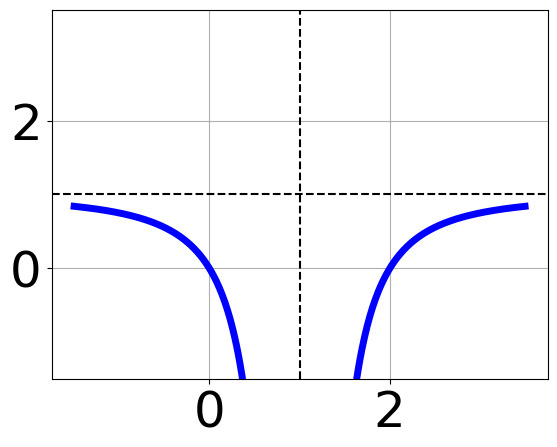
\includegraphics[width=0.5\textwidth]{../Figures/rationalGraphToEquationCopyA.png}
\end{center}
\begin{enumerate}[label=\Alph*.]
\item \( f(x) = \frac{1}{x - 1} + 1 \)
\item \( f(x) = \frac{-1}{x + 1} + 1 \)
\item \( f(x) = \frac{-1}{(x + 1)^2} + 1 \)
\item \( f(x) = \frac{1}{(x - 1)^2} + 1 \)
\item \( \text{None of the above} \)

\end{enumerate} }
\litem{
Choose the graph of the equation below.\[ f(x) = \frac{-1}{x - 3} + 3 \]\begin{enumerate}[label=\Alph*.]
\begin{multicols}{2}\item 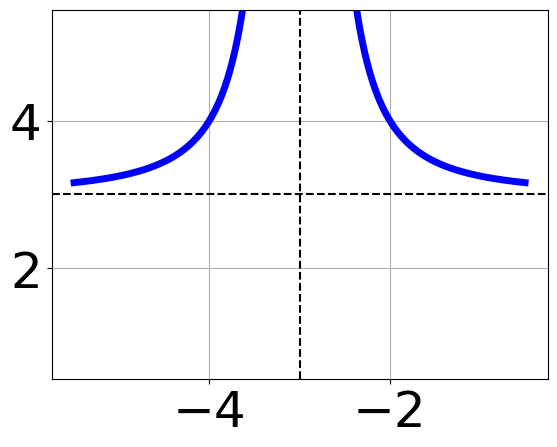
\includegraphics[width = 0.3\textwidth]{../Figures/rationalEquationToGraphCopyAA.png}\item 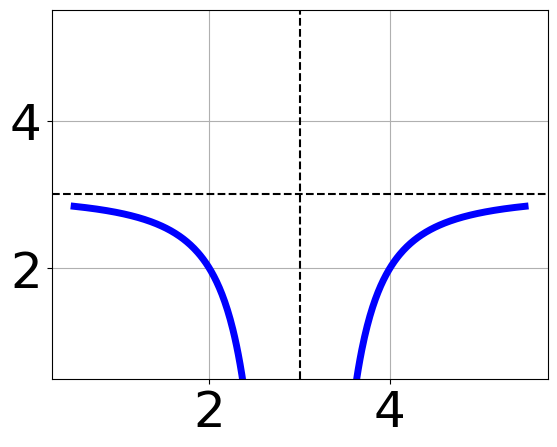
\includegraphics[width = 0.3\textwidth]{../Figures/rationalEquationToGraphCopyBA.png}\item 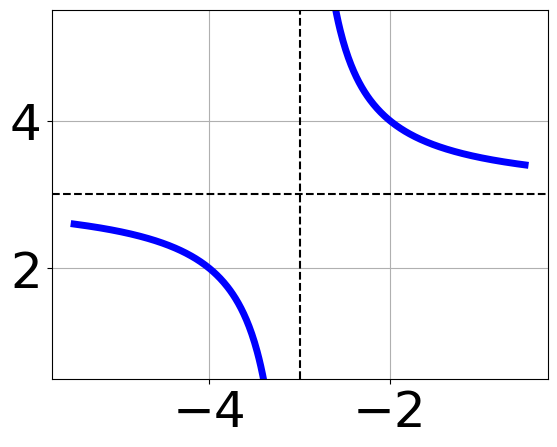
\includegraphics[width = 0.3\textwidth]{../Figures/rationalEquationToGraphCopyCA.png}\item 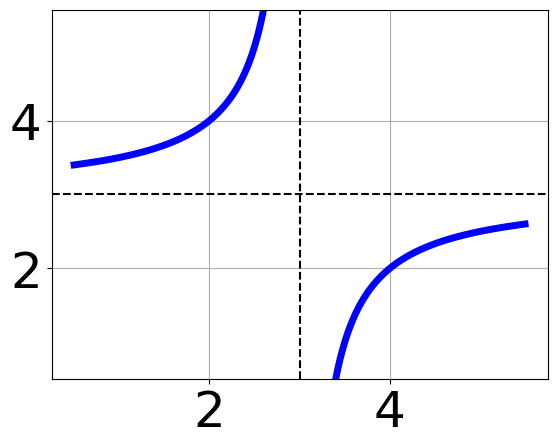
\includegraphics[width = 0.3\textwidth]{../Figures/rationalEquationToGraphCopyDA.png}\end{multicols}\item None of the above.
\end{enumerate} }
\litem{
Determine the domain of the function below.\[ f(x) = \frac{6}{18x^{2} -48 x + 30} \]\begin{enumerate}[label=\Alph*.]
\item \( \text{All Real numbers except } x = a \text{ and } x = b, \text{ where } a \in [0.08, 1.26] \text{ and } b \in [1.34, 2.24] \)
\item \( \text{All Real numbers.} \)
\item \( \text{All Real numbers except } x = a, \text{ where } a \in [14.2, 15.35] \)
\item \( \text{All Real numbers except } x = a, \text{ where } a \in [0.08, 1.26] \)
\item \( \text{All Real numbers except } x = a \text{ and } x = b, \text{ where } a \in [14.2, 15.35] \text{ and } b \in [35.49, 36.48] \)

\end{enumerate} }
\litem{
Solve the rational equation below. Then, choose the interval(s) that the solution(s) belongs to.\[ \frac{-3}{9x + 7} + 8 = \frac{-8}{-81x -63} \]\begin{enumerate}[label=\Alph*.]
\item \( x \in [0.7,0.98] \)
\item \( x \in [-1.72,1.28] \)
\item \( x_1 \in [-0.73, -0.57] \text{ and } x_2 \in [0.2,1.3] \)
\item \( \text{All solutions lead to invalid or complex values in the equation.} \)
\item \( x_1 \in [-1.11, -0.79] \text{ and } x_2 \in [-1.2,-0.2] \)

\end{enumerate} }
\litem{
Choose the graph of the equation below.\[ f(x) = \frac{-1}{(x + 3)^2} + 2 \]\begin{enumerate}[label=\Alph*.]
\begin{multicols}{2}\item 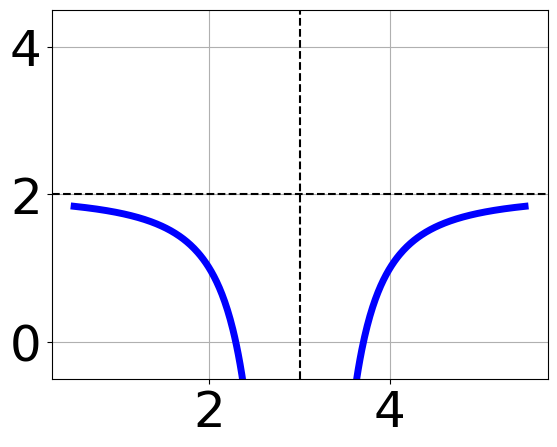
\includegraphics[width = 0.3\textwidth]{../Figures/rationalEquationToGraphAA.png}\item 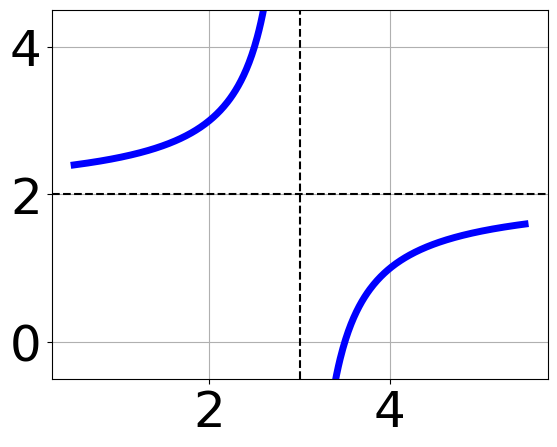
\includegraphics[width = 0.3\textwidth]{../Figures/rationalEquationToGraphBA.png}\item 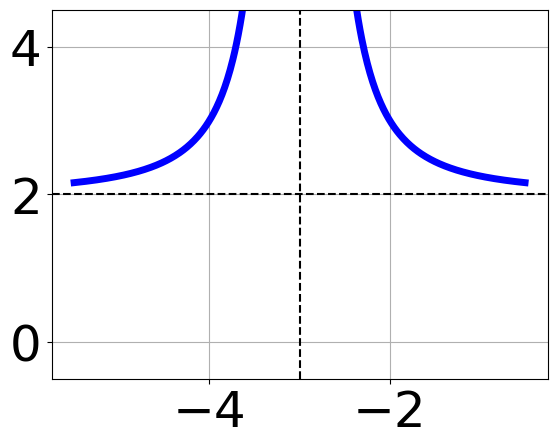
\includegraphics[width = 0.3\textwidth]{../Figures/rationalEquationToGraphCA.png}\item 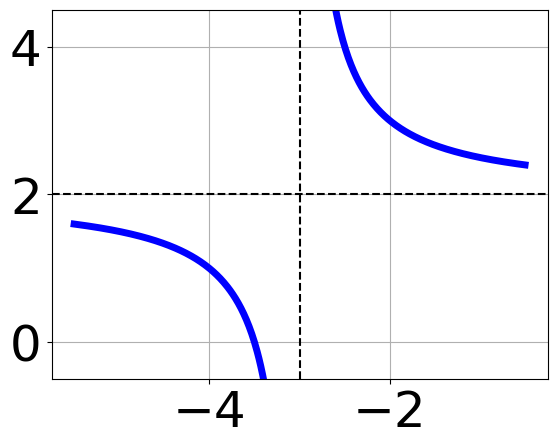
\includegraphics[width = 0.3\textwidth]{../Figures/rationalEquationToGraphDA.png}\end{multicols}\item None of the above.
\end{enumerate} }
\litem{
Choose the equation of the function graphed below.
\begin{center}
    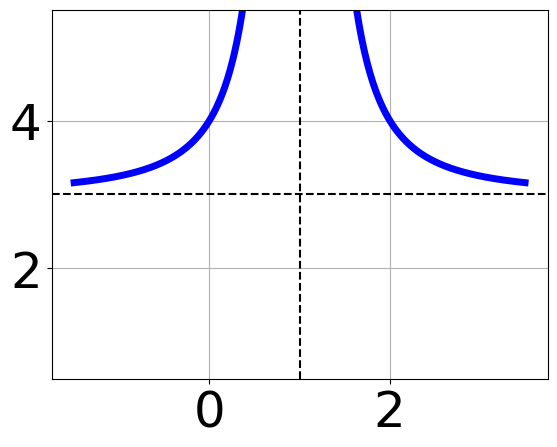
\includegraphics[width=0.5\textwidth]{../Figures/rationalGraphToEquationA.png}
\end{center}
\begin{enumerate}[label=\Alph*.]
\item \( f(x) = \frac{-1}{x + 1} + 3 \)
\item \( f(x) = \frac{-1}{(x + 1)^2} + 3 \)
\item \( f(x) = \frac{1}{(x - 1)^2} + 3 \)
\item \( f(x) = \frac{1}{x - 1} + 3 \)
\item \( \text{None of the above} \)

\end{enumerate} }
\litem{
Solve the rational equation below. Then, choose the interval(s) that the solution(s) belongs to.\[ \frac{-4x}{-6x -6} + \frac{-2x^{2}}{-12x^{2} +12 x + 24} = \frac{-3}{2x -4} \]\begin{enumerate}[label=\Alph*.]
\item \( x_1 \in [-1.52, -0.93] \text{ and } x_2 \in [0,4] \)
\item \( \text{All solutions lead to invalid or complex values in the equation.} \)
\item \( x \in [-1.52,-0.93] \)
\item \( x \in [1.74,3.27] \)
\item \( x_1 \in [1.03, 1.6] \text{ and } x_2 \in [-4.89,-0.89] \)

\end{enumerate} }
\litem{
Solve the rational equation below. Then, choose the interval(s) that the solution(s) belongs to.\[ \frac{3x}{5x -2} + \frac{-2x^{2}}{15x^{2} -26 x + 8} = \frac{-4}{3x -4} \]\begin{enumerate}[label=\Alph*.]
\item \( x \in [-3.37,0.31] \)
\item \( x \in [0.82,2.75] \)
\item \( x_1 \in [-0.86, 0.67] \text{ and } x_2 \in [0.4,2.4] \)
\item \( x_1 \in [-0.86, 0.67] \text{ and } x_2 \in [-4.78,0.22] \)
\item \( \text{All solutions lead to invalid or complex values in the equation.} \)

\end{enumerate} }
\end{enumerate}

\end{document}